\clearpage
\appendix

\section{Supplementary Figures}
\label{app:figures}

The figures below visualise the per-customer, per-band, per-year, and per-split diagnostics referenced from the main text.

\begin{figure*}[t]
    \centering
    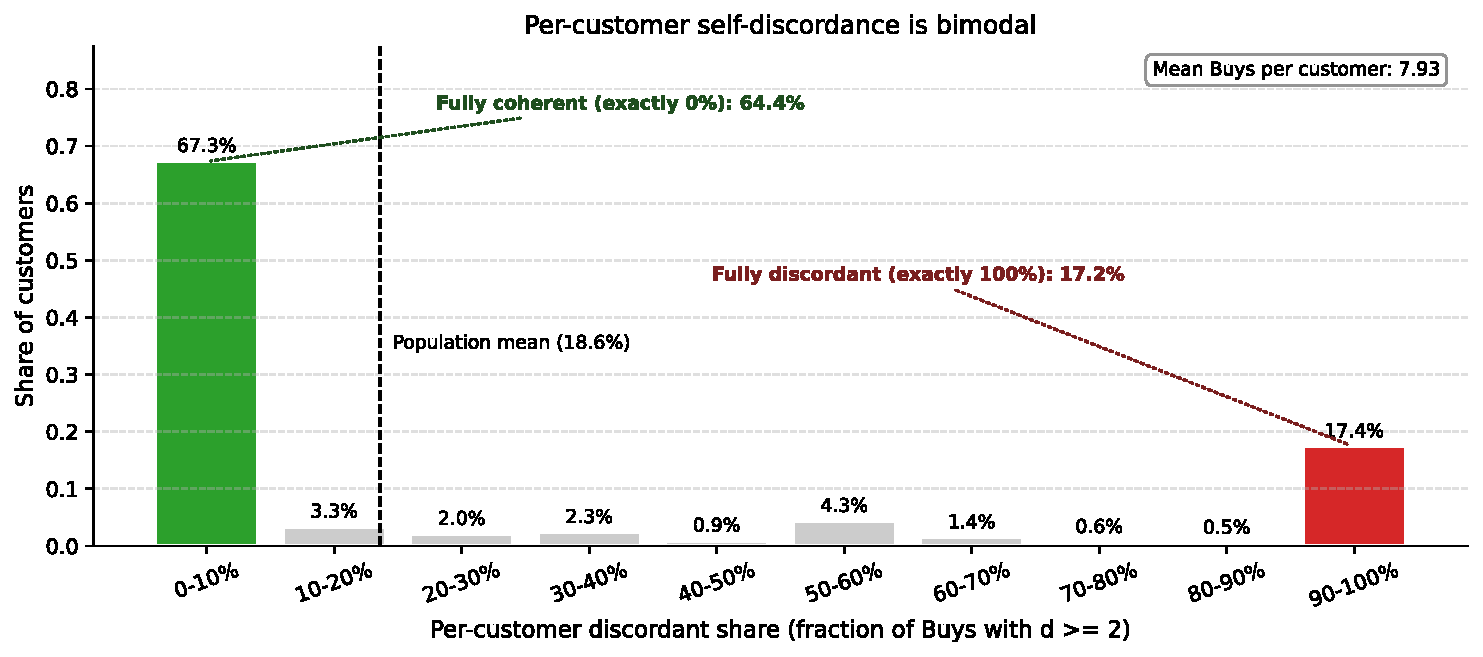
\includegraphics[width=\linewidth]{figures/rq1_self_discordance.pdf}
    \caption{Per-customer share of discordant Buys is sharply bimodal at 0\% and 100\%, ruling out i.i.d.\ transaction-level noise.}
    \label{fig:rq1-self}
\end{figure*}

\begin{figure*}[t]
    \centering
    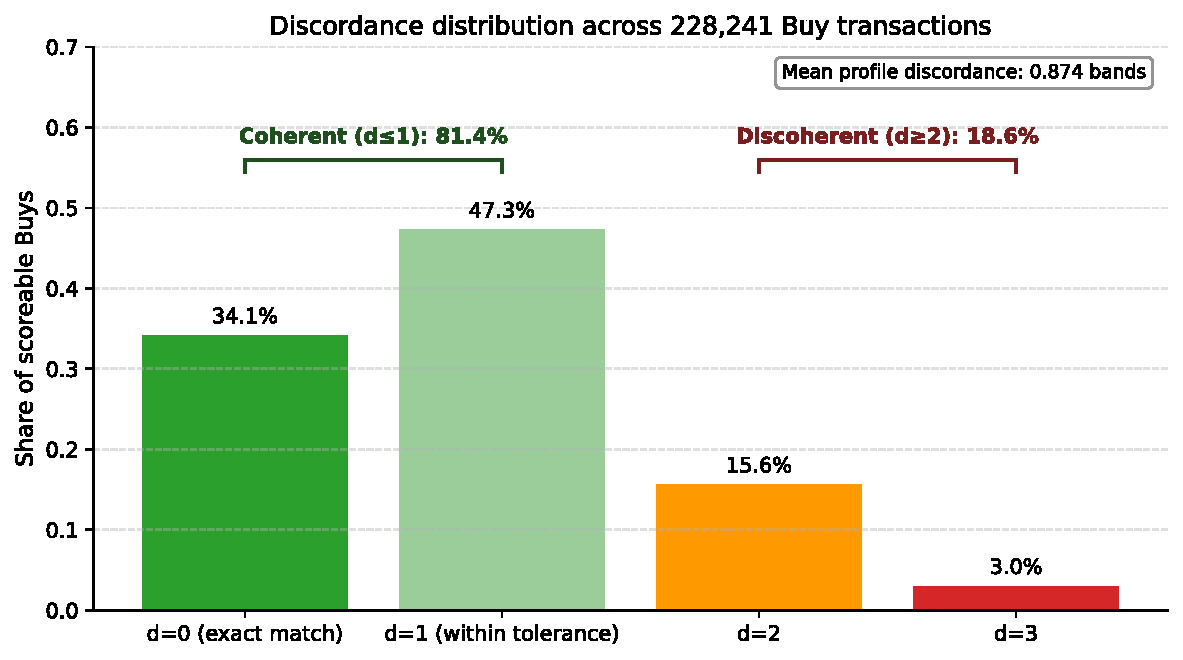
\includegraphics[width=\linewidth]{figures/rq1_discordance_distribution.pdf}
    \caption{Distribution of pairwise discordance $d$ over 228{,}241 scoreable Buys. The shape is heavy-tailed, with the typical violation being a one-band miss.}
    \label{fig:rq1-dist}
\end{figure*}

\begin{figure*}[t]
    \centering
    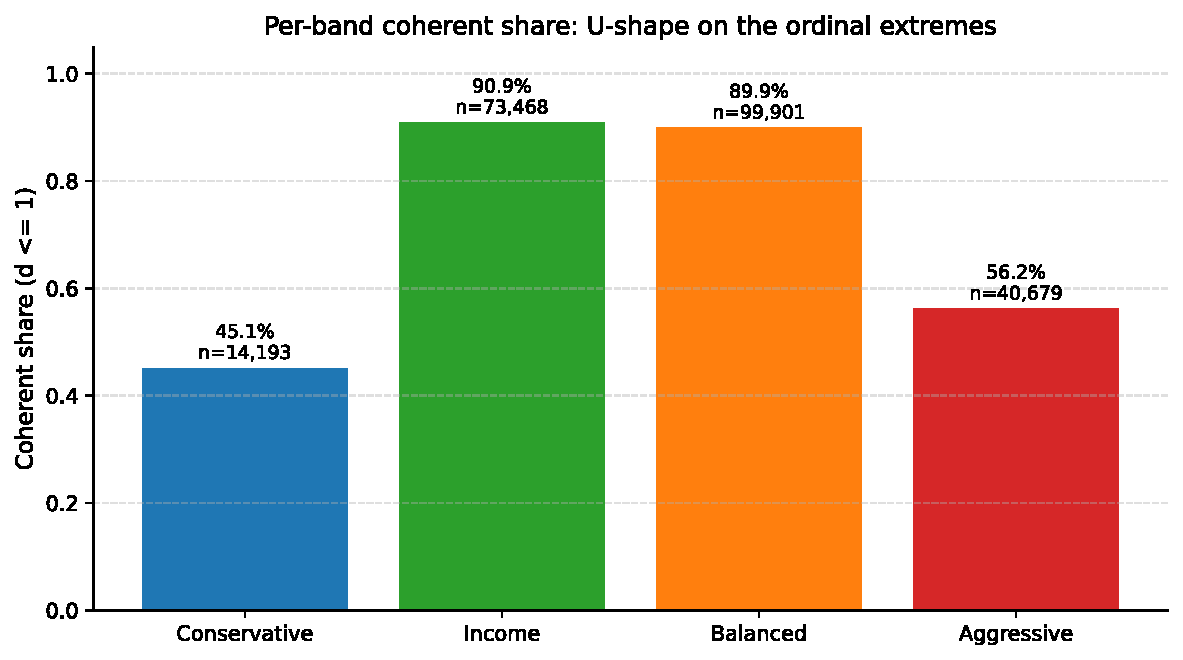
\includegraphics[width=\linewidth]{figures/rq1_per_band_coherence.pdf}
    \caption{Coherence share by declared band. The U-shape supports the bimodality result of Figure~\ref{fig:rq1-self}: discordance concentrates on the ordinal extremes.}
    \label{fig:rq1-per-band}
\end{figure*}

\begin{figure*}[t]
    \centering
    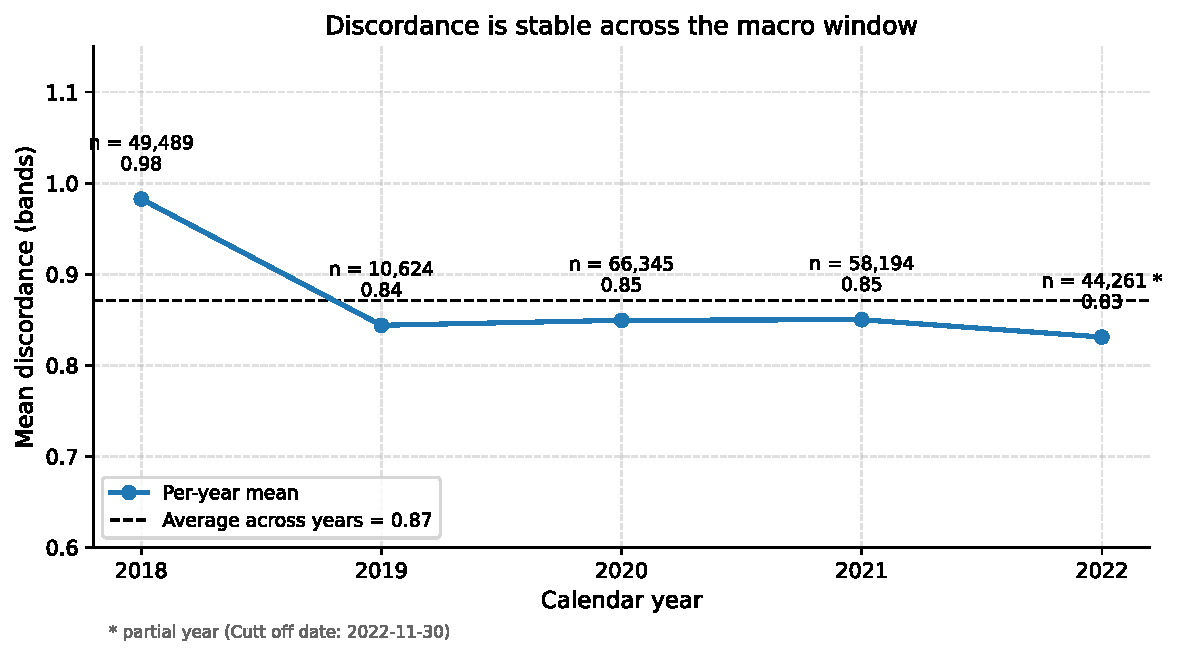
\includegraphics[width=\linewidth]{figures/rq1_yearly_discordance.pdf}
    \caption{Mean discordance by calendar year. The 2019 to 2022 cluster sits within 0.02 bands, with 2018 elevated (transition-effect hypothesis).}
    \label{fig:rq1-yearly}
\end{figure*}

\begin{figure*}[t]
    \centering
    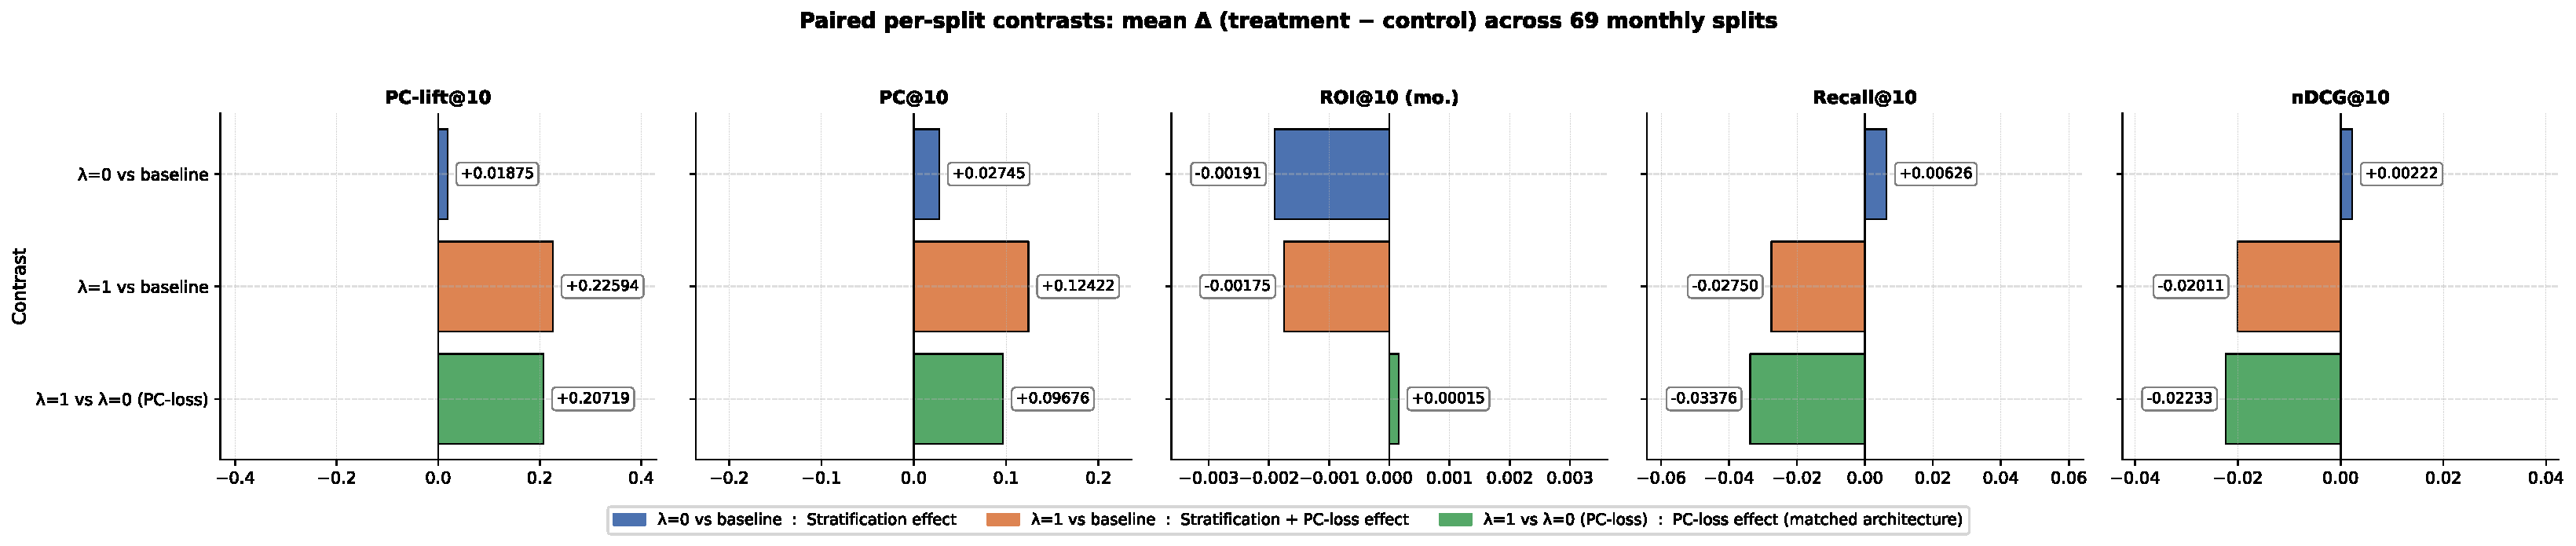
\includegraphics[width=\linewidth]{figures/rq4_paired_deltas.pdf}
    \caption{Paired per-split deltas of $\lambda = 1$ vs baseline LightGCN. PC@10 is positive on every one of 69 splits.}
    \label{fig:rq4-deltas}
\end{figure*}

\begin{figure*}[t]
    \centering
    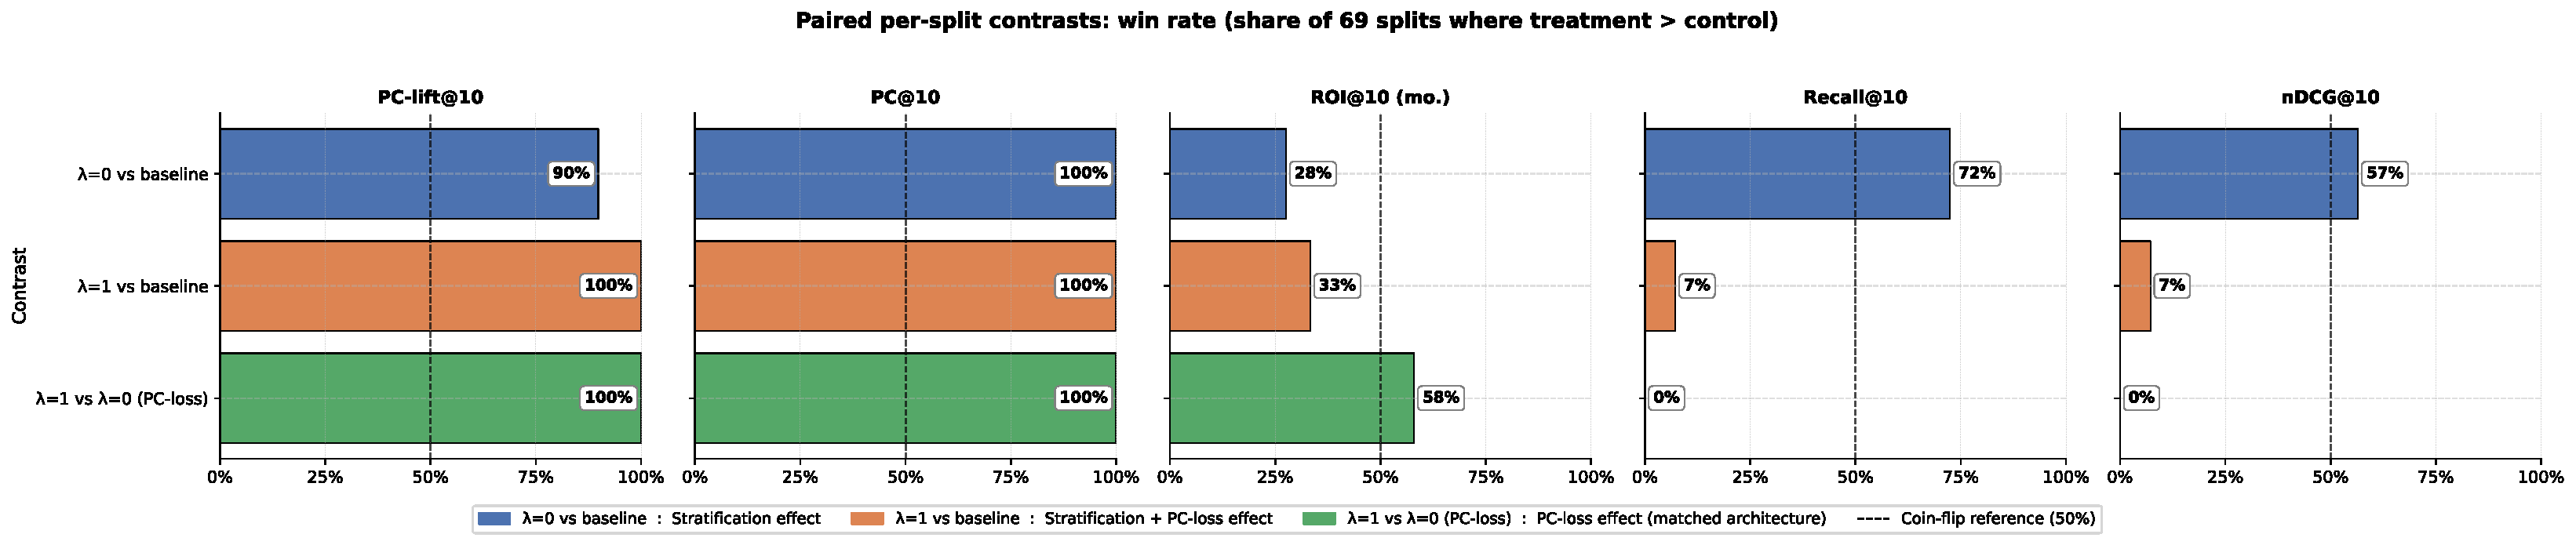
\includegraphics[width=\linewidth]{figures/rq4_paired_win_rates.pdf}
    \caption{Per-split win rates of the $\lambda = 0$ and $\lambda = 1$ trials against the global LightGCN baseline.}
    \label{fig:rq4-winrate}
\end{figure*}
